%%%%%%%%%%%%%%%%%%%%%%%%%%%%%%%%%%%%%%%%%%%%%%%%%%%%
\documentclass[fleqn,10pt,twocolumn]{AROB}

\usepackage[utf8]{inputenc}
\usepackage{amsmath}
\usepackage{xeCJK}
\usepackage{svg}
\setCJKmainfont{Hiragino Mincho ProN}

\title{可視カメラ 30fps 環境の PPG に最適化した\\
非対称サイン波モデルに基づく血圧推定}

\author{中澤 祐介${}^{1\dagger}$,南雲健人${}^{1}$,野澤昭雄${}^{1}$}
% The dagger symbol indicates the presenter.
\speaker{中澤 祐介}

\affils{${}^{1}$青山学院大学大学院理工学研究科 電気電子工学専攻\\
(Tel: 080-5326-3916; E-mail: nynynakazawa@gmail.com)\\
}

\abstract{%
スマートフォン可視カメラ由来の擬似PPGに対し、周波数分解に依存しない新規な血圧推定手法を提案する。30fpsという低サンプリングレート環境において、従来の周波数解析アプローチは高次高調波の正確な抽出が困難である。本研究では、既存の形態学的特徴量アプローチ(RTBP:RealTimeBloodPressure)をベースラインとして採用し、新規に提案する2つの手法を実装し、比較する。第一に、sin波フィットのパラメータ(振幅、位相、平均値)を直接特徴量として使用した線形回帰モデル(sinBP(M): sinBP(Model))である。第二に、生理学的に妥当な非対称サイン波モデルからの残差(歪み指標E)を特徴量として使用した3段階推定モデル(sinBP(D): sinBP(Distortion))である。sinBP(M)とsinBP(D)は、PPG波形の本質的な特性を抽出し、ノイズの影響を受けにくい安定した血圧推定を実現する。本研究の評価は、連続血圧計を参照として、30fps可視カメラのrPPG環境を使用した3つの異なる血圧推定手法(RTBP、sinBP(M)、sinBP(D))を比較し、新規手法の優位性を検証する。
}

\keywords{%
血圧推定、光電容積脈波、スマートフォン、非対称サイン波モデル、歪み指標
}

\begin{document}

\maketitle

%-----------------------------------------------------------------------

\section{序論}

連続的な非侵襲血圧モニタリングは、心血管疾患の早期発見・管理に不可欠である\cite{ref1,ref2}。近年、スマートフォンの可視カメラを用いた光電容積脈波(PPG)による非侵襲かつ簡易的な血圧推定が注目されている\cite{ref3}。

一般に、PPG波形の特徴量は生理学的な血管特性を反映する。例えば、振幅(A)は血管のしなやかさ(伸展性)や血液の拍出量を反映し\cite{ref3,ref4}、心拍数(HR)は自律神経活動を反映する。また、波形の鋭さを示す相対TTP(脈波周期に対するピーク到達時間の割合)は、血管が硬くなるほど反射波が早期に戻る現象(脈波伝播速度の上昇)を捉え、動脈硬化の指標となる\cite{ref5,ref6}。これらのPPG特徴量と血圧には線形関係が存在することが示されている\cite{ref5,ref7,ref8}。従来のPPG血圧推定は、これらの特徴量を(1)形態学的特徴量(ピーク、TTP等)\cite{ref5}、(2)周波数解析(FFT等)\cite{ref9}、(3)機械学習(深層学習等)\cite{ref10}といった手法で抽出してきた。

しかし、スマホカメラは30fpsと脈波を測定するにはサンプリングレートが低く、照明変動や体動由来のノイズの影響を受けやすい。この環境下では、微細な特徴点(ピーク位置やTTP(Time To Peak/脈波の立ち上がりからピークに達するまでの時間)など)に依存する形態学的解析は不安定となり、周波数の制約から周波数解析も困難である\cite{ref11,ref12}。

これに対して本研究では、局所的な特徴点や周波数成分ではなく、「波形全体の形状(Shape)」に着目する。1拍分の全データポイントを用いてモデル関数にフィットさせることにより、局所的なノイズやサンプリングのズレを平滑化できるため、30fpsという低サンプリングレート・高ノイズ環境においてもロバストな特徴抽出が可能であると仮説を立てた。

具体的には、収縮期・拡張期の非対称性を考慮した非対称サイン波モデルを提案する。一般に、PPG波形はガンマ関数やベータ関数、あるいは歪度を持つガウシアンモデルなどで表現可能と報告されているが\cite{ref13,ref14}、これらは多数のパラメータを必要とし、計算コストが高いことに加え、特に低サンプリングレート環境においてノイズの影響を受けやすく安定性に乏しいという課題がある。対して、本提案モデルは、PPG特有の急峻な立ち上がりと緩やかな減衰\cite{ref4}を、収縮期と拡張期の時間比率($\alpha$)という単一のパラメータで表現する。これにより、最小限のパラメータ数(振幅、位相、平均、$\alpha$)で波形の主要な特徴を捉えることができ、30fpsの低サンプリングレート環境においても計算コストが低く、かつロバストな推定が可能である。

本研究の目的は、この非対称サイン波モデルを用いた新規手法の有効性を、従来手法と比較検証することである。具体的には、以下の構成で比較を行う。
(1) 従来手法(RTBP): 既存のPPG波形の形態学的特徴量(振幅、心拍数、相対TTP)を用いる手法\cite{ref5}。これをベースラインとする。
(2) 提案手法(非対称サイン波モデル):
(2-1) モデルパラメータ活用法(sinBP(M)): 既存のPPG波形への適合により得られる非対称サイン波モデルのパラメータ(振幅、位相、平均値)を特徴量とする手法。
(2-2) 従来手法と提案モデルの組み合わせ(sinBP(D)): 従来手法(RTBP)と非対称サイン波モデルを組み合わせた手法。本研究では、組み合わせの一例として、RTBPの特徴量にモデル残差を追加する手法を検討する。

なお、全手法において、各特徴量を説明変数、血圧値を目的変数とし、多重共線性を考慮した正則化項を持つRidge回帰を採用する\cite{ref15}。

本研究の主な貢献は、30fpsの低品質な映像環境においても安定した特徴抽出を可能にする「非対称サイン波モデル適合手法」を提案した点である。点計測に依存する従来手法(RTBP)に対し、波形形状全体を利用することでノイズへの頑健性を高めるアプローチである。

%-----------------------------------------------------------------------

\section{手法}

\subsection{非対称サイン波モデル}
PPG波形は、収縮期(立ち上がり)が短く拡張期(立ち下がり)が長い非対称性を有する\cite{ref16}。本研究では、実測波形$x[n]$に対し、この特性を反映した非対称サイン波モデル$s(t)$を最小二乗法によりフィッティングさせる。モデルは、波形の収縮期と拡張期を異なる周波数の正弦波で表現する(式\ref{eq:asymmetric_model})。

\begin{equation}
s(t) = \text{mean} + \frac{A}{2} \cdot \sin(\theta(t))
\label{eq:asymmetric_model}
\end{equation}

\begin{equation}
\theta(t) = \begin{cases}
-\frac{\pi}{2} + \pi \cdot \frac{t'}{T_{sys}} & (0 \leq t' < T_{sys}) \quad [\text{立ち上がり}] \\
\frac{\pi}{2} + \pi \cdot \frac{t' - T_{sys}}{T_{dia}} & (T_{sys} \leq t' < T) \quad [\text{立ち下がり}]
\end{cases}
\label{eq:asymmetric_theta}
\end{equation}

ここで、$A$は振幅、meanは平均値、$T$は周期(IBI)である。$T_{sys}$は収縮期時間、$T_{dia}$は拡張期時間であり、$T = T_{sys} + T_{dia}$の関係にある。$t'$は各拍の開始点(谷)を基準とした時刻であり、$t' = (t - \tau_{foot}) \bmod T$で表される($\tau_{foot}$は位相ズレ補正項)。立ち上がり区間ではsinが$-1 \to 1$(谷$\to$ピーク)へ推移し、立ち下がり区間では$1 \to -1$(ピーク$\to$谷)へ推移することで、PPG特有の非対称な拍動波形を形成する。

本研究では、実測データから収縮期/拡張期比率($\alpha = T_{sys}/T$)を計算し、その比率に基づいて動的にモデルパラメータを決定する。初期値として$\alpha = 1/3 (T_{sys} = T/3, T_{dia} = 2T/3)$を設定する。

\subsection{特徴量抽出}
本研究では、以下の3つの観点から特徴量を抽出する。

(1) 形態学的特徴量 従来手法(RTBP)で用いられる基本的な特徴量である。
\begin{itemize}
\item 振幅(A): 波形のAC成分の大きさ。血管の伸展性を反映する。
\item 心拍数(HR): 1分間あたりの拍動数。自律神経活動を反映する。
\item 相対TTP: 脈波周期に対する立ち上がり時間の割合(V2P\_relTTP)および立ち下がり時間の割合(P2V\_relTTP)。血管硬化度を反映する。
\end{itemize}

(2) モデルパラメータ 非対称サイン波モデルへの適合により得られるパラメータである。
\begin{itemize}
\item 振幅(A): モデルの振幅項。
\item 平均値(Mean): 波形のDC成分。
\item 位相($\Phi$): 波形の位相ズレ。
\end{itemize}

(3) モデル残差特徴量 実測波形$x[n]$とモデル波形$s[n]$の乖離度を表す特徴量である。まず、RMS誤差を残差$E$として定義する(式\ref{eq:distortion})。

\begin{equation}
E = \sqrt{\frac{1}{N} \sum_{n=1}^{N} (x[n] - s[n])^2}
\label{eq:distortion}
\end{equation}

さらに、振幅と残差の相互作用を考慮した項($E\sqrt{A}$)も定義する。

\begin{equation}
\text{Stiffness}_{\text{sin}} = E \sqrt{A}
\label{eq:stiffness}
\end{equation}

\subsection{血圧推定プロセス}
\subsubsection{前処理}
ピーク検出、ビート切り出し、時間正規化($N=64$)、ピーク整合(位相探索)、外れ値除去(IBI, 振幅変動)を実施する。

\subsubsection{推定モデル構築}
抽出した特徴量を用いて、以下の3つの血圧推定モデルを構築する。全手法において、各特徴量を説明変数、血圧値を目的変数とし、多重共線性を考慮した正則化項を持つRidge回帰を採用する\cite{ref15}。

(1) 従来手法(RTBP) 形態学的特徴量のみを用いるモデルである。説明変数として、振幅$A$、心拍数HR、および相対TTP(V2P\_relTTP, P2V\_relTTP)を使用する。

(2) モデルパラメータ活用法(sinBP(M)) モデルパラメータを特徴量とするモデルである。説明変数として、振幅$A$、心拍数HR、平均値Mean、位相$\Phi$を使用する。

(3) 従来手法と提案モデルの組み合わせ(sinBP(D)) RTBPの特徴量に加え、モデル残差特徴量を追加したモデルである。推定は以下の2段階で行う。
1. ベースBP+血管特性補正: RTBPの特徴量に加え、血管硬化指標Stiffness\_{sin}を説明変数として推定を行う。
2. 歪み補正: 第1段階の推定値に対し、残差$E$を説明変数として補正を行う。

%-----------------------------------------------------------------------

\section{実験計画}
\subsection{実験環境}
環境設定
デバイスにはGoogle Pixel 8のフロント可視カメラ(30fps)を使用し、指腹接触方式(第2指)で測定を行った。照明条件は室内400 luxとした。

参照値
参照デバイスとして、指先カフ(第3指)で実時間PPGを光学式パルスオキシメーター(IWS920-DEV 分解能409.6Hz)で同時計測した。また、指先カフ(第3指/第4指)で実時間血圧を連続血圧計(CNAP-Monitor 分解能1000Hz 臨床グレード)で同時計測した。測定条件として、測定間隔・体位・安静時間を統一した。

被験者
被験者は20~23歳の健康な成人男性5名であり、不整脈重度等の除外条件を設けた。各被験者につき3回ずつ計測を行った。

倫理的配慮
本実験はヘルシンキ宣言に基づき実施され、所属機関の倫理委員会の承認を得ている。全被験者から事前に書面によるインフォームド・コンセントを取得し、収集したデータは個人が特定されないよう匿名化し、暗号化して保存された。

\subsection{実験手順}
被験者は椅子に座り、安静状態を保った。左手の中指にCNAPの指カフを装着し、右手の人差し指をスマートフォンのカメラに軽く接触させた。実験は以下の手順で行った。
1. 安静計測(60秒): 自然な呼吸で安静状態を維持。
2. 深呼吸(60秒): 5秒吸気・5秒呼気のペースで深呼吸を行い、血圧変動を誘発。
3. 回復(60秒): 再び自然な呼吸で安静状態に戻る。
計180秒間のデータを1セッションとし、各被験者に対し複数回実施した。

\subsection{評価指標}
本研究では以下の指標を用いて評価を行う。まず波形評価として、スマートフォンカメラのGreenチャンネルから取得した生PPG波形(以下、Green)およびに提案手法により生波形にフィッティングされた近似波形(以下、sinWave)を、参照波形と時間同期し、MAPE、MAE、相関係数で評価する。次に血圧推定精度については、5分割時系列交差検証を用い、MAE, RMSE, MAPEで3手法を比較検証する。その際、AAMI基準($|\text{MD}|\leq 5, \text{SD}\leq 8$)も参照する。さらにアブレーションとして、各特徴量の寄与を係数分析により評価する。

\section{結果}
\subsection{波形評価}
表\ref{tab:waveform_eval}に波形評価結果を示す。sinWaveはGreenと比較してMAPEで約11.5ポイント改善し、相関係数も向上した。これはモデル近似がノイズ除去として機能したことを示す。

\begin{table}[h]
\caption{Waveform evaluation results (Average of all sessions)}
\label{tab:waveform_eval}
\centering
\small
\begin{tabular}{lccccc}
\hline
Channel & MAPE [\%] & MAE & RMSE & Bias & Corr \\
\hline
sinWave & 18.22 & 1.82 & 2.24 & -0.66 & 0.19 \\
Green & 29.71 & 2.97 & 3.64 & +0.42 & 0.07 \\
\hline
\end{tabular}
\end{table}

\subsection{血圧推定精度}
表\ref{tab:sbp_acc}, \ref{tab:dbp_acc}に推定精度を示す。提案手法sinBP(D)がSBP/DBP共に最小のMAE/RMSEを達成した。特にRMSEの改善が顕著であり、大きな誤差を抑制できている。図\ref{fig:sbp_ba_all}, \ref{fig:dbp_ba_all}にBland-Altmanプロットを示す。RTBPと比較して、提案手法ではバイアスが低減し、一致限界の幅も狭まっていることが確認できる。また、図\ref{fig:sbp_comp}, \ref{fig:dbp_comp}に各手法の精度の比較を示す。

\begin{table}[h]
\caption{SBP estimation accuracy}
\label{tab:sbp_acc}
\centering
\small
\begin{tabular}{lccc}
\hline
Method & MAPE [\%] & MAE [mmHg] & RMSE [mmHg] \\
\hline
RTBP & 17.82 & 20.66 & 28.02 \\
sinBP(M) & 16.92 & 19.47 & 24.70 \\
sinBP(D) & 16.44 & 18.98 & 24.17 \\
\hline
\end{tabular}
\end{table}

\begin{table}[h]
\caption{DBP estimation accuracy}
\label{tab:dbp_acc}
\centering
\small
\begin{tabular}{lccc}
\hline
Method & MAPE [\%] & MAE [mmHg] & RMSE [mmHg] \\
\hline
RTBP & 23.14 & 16.11 & 22.43 \\
sinBP(M) & 22.30 & 15.20 & 19.73 \\
sinBP(D) & 21.72 & 14.84 & 19.31 \\
\hline
\end{tabular}
\end{table}

\begin{figure*}[t]
\centering
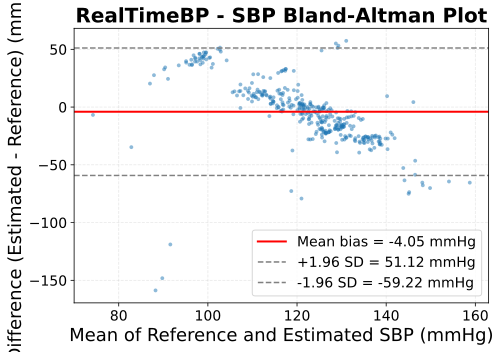
\includegraphics[width=0.32\textwidth]{figures/RealTimeBP_SBP_bland_altman.png}
\hfill
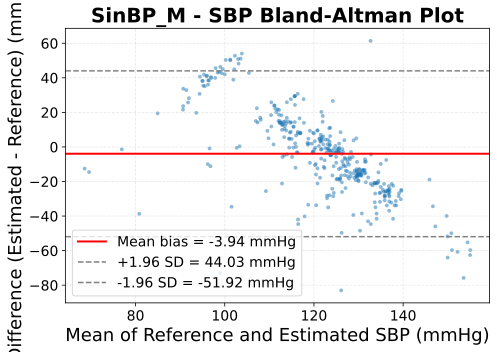
\includegraphics[width=0.32\textwidth]{figures/SinBP_M_SBP_bland_altman.png}
\hfill
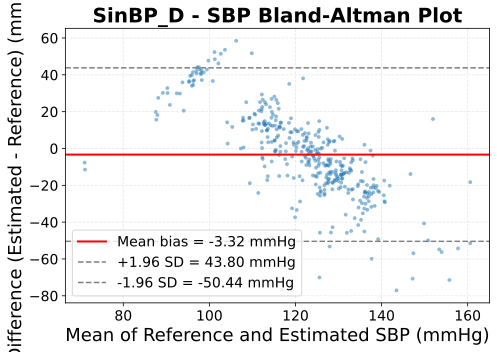
\includegraphics[width=0.32\textwidth]{figures/SinBP_D_SBP_bland_altman.png}
\caption{Bland-Altman plots of SBP. Left: RTBP, Center: sinBP(M), Right: sinBP(D).}
\label{fig:sbp_ba_all}
\end{figure*}

\begin{figure*}[t]
\centering
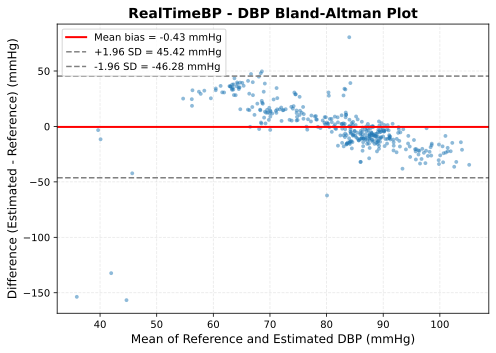
\includegraphics[width=0.32\textwidth]{figures/RealTimeBP_DBP_bland_altman.png}
\hfill
\includegraphics[width=0.32\textwidth]{figures/SinBP_M_DBP_bland_altman.png}
\hfill
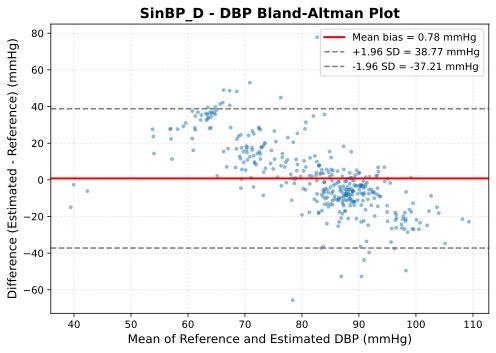
\includegraphics[width=0.32\textwidth]{figures/SinBP_D_DBP_bland_altman.png}
\caption{Bland-Altman plots of DBP. Left: RTBP, Center: sinBP(M), Right: sinBP(D).}
\label{fig:dbp_ba_all}
\end{figure*}

\begin{figure}[t]
\centering
\includegraphics[width=0.49\linewidth]{figures/comparison_SBP_barplot_MAE.png}
\hfill
\includegraphics[width=0.49\linewidth]{figures/comparison_SBP_barplot_RMSE.png}
\\[0.5em]
\includegraphics[width=0.49\linewidth]{figures/comparison_SBP_barplot_MAPE.png}
\caption{Comparison of SBP estimation accuracy across three methods (RTBP, sinBP(M), sinBP(D)). Top left: MAE, Top right: RMSE, Bottom: MAPE.}
\label{fig:sbp_comp}
\end{figure}

\begin{figure}[t]
\centering
\includegraphics[width=0.49\linewidth]{figures/comparison_DBP_barplot_MAE.png}
\hfill
\includegraphics[width=0.49\linewidth]{figures/comparison_DBP_barplot_RMSE.png}
\\[0.5em]
\includegraphics[width=0.49\linewidth]{figures/comparison_DBP_barplot_MAPE.png}
\caption{Comparison of DBP estimation accuracy across three methods (RTBP, sinBP(M), sinBP(D)). Top left: MAE, Top right: RMSE, Bottom: MAPE.}
\label{fig:dbp_comp}
\end{figure}

sinBP(D)における特徴量の寄与:
sinBP(D)では、歪み指標$E$がSBP・DBPともに大きな正の係数(SBP: +14.88, DBP: +15.20)を持っていた。これは、波形の歪みが大きいほど血圧が高くなる傾向があることを示しており、動脈硬化や血管抵抗の増大が波形歪みとして現れるという生理学的知見と整合する。
一方、血管硬さ指標Stiffness\_sin ($E\sqrt{A}$)は負の係数(SBP: -2.40, DBP: -3.44)を示した。これは単独の歪みだけでなく、振幅との相互作用項が補正として機能していることを示唆する。

sinBP(M)における特徴量の寄与:
sinBP(M)では、位相Phiが正の係数(SBP: +11.79, DBP: +15.69)を持ち、血圧推定に大きく寄与していることが確認された。これは、脈波の伝播速度や反射波のタイミング(位相)が血圧と密接に関連していることを裏付けている。

\section{考察}

\subsection{結果の解釈}

本研究の結果は、30fpsという低サンプリングレート環境において、周波数解析に依存しない非対称サイン波モデルによる近似アプローチが有効であることを強く支持している。

まず、波形評価においてsinWaveチャンネルがGreenチャンネルよりも高い精度(低MAPE)を示したことは、非対称サイン波モデルがノイズ除去と波形整形フィルタとして機能し、PPGの基本成分を抽出できていることを意味する。生のGreen信号は照明変動や体動ノイズの影響を直接受けるが、モデル近似を行うことで、生理学的に妥当な「理想波形」への回帰が行われ、S/N比が向上したと考えられる。

次に、血圧推定においてsinBP(D)が最高精度を達成したことは、「生理学的モデルからの逸脱(残差)」が血圧推定において重要な情報を持っていることを示している。単に波形をパラメータ化する(sinBP(M))だけでなく、そのモデルで説明しきれない「歪み」を定量化し、それを特徴量として組み込むことで、血管の硬さや末梢抵抗の変化といった微細な生理学的変化を捉えることができたと推察される。

\subsection{手法の優位性}

既存手法(RTBP)は、波形のピークや谷といった「点」の情報に依存するため、30fpsの粗い時間分解能では正確な特徴抽出が困難であった(サンプリング点がピークからずれる等)。これに対し、提案手法(sinBPシリーズ)は、1拍分の全データポイントを用いた最小二乗フィットを行うため、サンプリングタイミングのずれに対して頑健である。これが、sinBP(M)およびsinBP(D)がRTBPを上回る精度を出した主要因と考えられる。

さらに、sinBP(D)がsinBP(M)を上回った事実は、非対称サイン波モデルという「生理学的制約」の有効性を示している。単なるパラメータ抽出(sinBP(M))よりも、収縮期・拡張期の比率を考慮した非対称モデルの残差($E$)の方が純粋な「病的/生理的歪み」を反映するようになったため、血圧との相関が高まったと考えられる。

\subsection{限界と展望}
MAPEは16\%台であり、AAMI基準には達していない。今後は、(1)個人差補正(キャリブレーション)、(2)モデル拡張(第2高調波追加)、(3)データセット拡充に取り組む必要がある。

\section{結論}
本研究では、30fps可視カメラ環境向けに、非対称サイン波モデルを用いた血圧推定手法を提案した。実験の結果、モデル残差を用いたsinBP(D)が最も高い精度を示し、血管硬化を反映する歪み指標の有効性が確認された。

本研究の主な貢献は、30fpsの低品質な映像環境においても安定した特徴抽出を可能にする「非対称サイン波モデル適合手法」を提案した点である。点計測に依存する従来手法(RTBP)に対し、波形形状全体を利用することでノイズへの頑健性を高めるアプローチである。

本手法は、専用デバイスを必要としない手軽な血圧モニタリング技術として、モバイルヘルス分野への貢献が期待される。今後は、個人差補正の導入や大規模データセットでの検証を進め、実用化を目指す。

%%%%%%%%%%%%%%%%% BIBLIOGRAPHY IN THE LaTeX file !!!!! %%%%%%%%%%%%%%%%%%%%%%
\begin{thebibliography}{16}
\bibitem{ref1}
World Health Organization. "Global report on hypertension 2023: the race against a silent killer." Geneva: World Health Organization, 2023.

\bibitem{ref2}
Whelton, Paul K., et al. "2017 ACC/AHA Guideline for the Prevention, Detection, Evaluation, and Management of High Blood Pressure in Adults." \textit{Journal of the American College of Cardiology}, vol. 71, no. 19, 2018, pp. e127-e248.

\bibitem{ref3}
Sun, Yu, and Nitish Thakor. "Photoplethysmography revisited: from contact to noncontact, from point to imaging." \textit{IEEE Transactions on Biomedical Engineering}, vol. 63, no. 3, 2016, pp. 463-477.

\bibitem{ref4}
Allen, John. "Photoplethysmography and its application in clinical physiological measurement." \textit{Physiological Measurement}, vol. 28, no. 3, 2007, pp. R1-R39.

\bibitem{ref5}
Millasseau, Sandrine C., et al. "Contour analysis of the photoplethysmographic pulse measured at the finger." \textit{Journal of Hypertension}, vol. 24, no. 8, 2006, pp. 1449-1456.

\bibitem{ref6}
Nichols, Wilmer W. "Clinical measurement of arterial stiffness obtained from noninvasive pressure waveforms." \textit{American Journal of Hypertension}, vol. 18, no. 1, 2005, pp. 3S-10S.

\bibitem{ref7}
Charlton, Peter H., et al. "Assessing model age from the photoplethysmogram: a systematic review." \textit{IEEE Reviews in Biomedical Engineering}, vol. 12, 2019, pp. 179-202.

\bibitem{ref8}
Elgendi, Mohamed. "On the analysis of fingertip photoplethysmogram signals." \textit{Current Cardiology Reviews}, vol. 8, no. 1, 2012, pp. 14-25.

\bibitem{ref9}
Alian, Aymen A., and Kirk H. Shelley. "Photoplethysmography." \textit{Best Practice \& Research Clinical Anaesthesiology}, vol. 28, no. 4, 2014, pp. 395-406.

\bibitem{ref10}
Zhang, Liang, et al. "Developing personalized models of blood pressure estimation from wearable sensors data using minimally-trained domain adversarial neural networks." \textit{Proceedings of Machine Learning Research}, vol. 126, 2020, pp. 97-120.

\bibitem{ref11}
Verkruysse, Wim, Lars O. Svaasand, and J. Stuart Nelson. "Remote plethysmographic imaging of skin perfusion." \textit{Optics Express}, vol. 16, no. 26, 2008, pp. 21434-21445.

\bibitem{ref12}
McDuff, Daniel, et al. "Improvements in remote cardiopulmonary measurement using a five band camera." \textit{IEEE Transactions on Biomedical Engineering}, vol. 61, no. 10, 2014, pp. 2593-2601.

\bibitem{ref13}
Basso, G., Haakma, R., and Vullings, R., "A skewed-Gaussian model for pulse decomposition." \textit{Physiological Measurement}, vol. 45, no. 11, 2024.

\bibitem{ref14}
Tiinanen, T., Popa, A.-G., Käpylä, M., and Fränti, A., "Model selection for the pulse decomposition analysis of fingertip photoplethysmograms." \textit{Proc. IEEE Eng. Med. Biol. Soc. (EMBC)}, 2017, pp. 1624-1627.

\bibitem{ref15}
Mukkamala, Ramakrishna, et al. "Toward ubiquitous blood pressure monitoring via pulse transit time: theory and practice." \textit{IEEE Transactions on Biomedical Engineering}, vol. 62, no. 8, 2015, pp. 1879-1901.

\bibitem{ref16}
Hall, John E., and Michael E. Hall. \textit{Guyton and Hall Textbook of Medical Physiology}. 14th ed., Elsevier, 2020.
\end{thebibliography}

\end{document}
